\chapter{Autoencoders}

\section{Motivation}

All algorithms up to this point have \textbf{required data with ground truth and utilized supervised learning}. This \textbf{inductive bias} has come with a list of challenges: 

\begin{itemize}
    \item \textbf{Requires large amounts of labeled data}
    \item \textbf{Obtaining labeled data is expensive} → people need to be hired to label data
    \item \textbf{Medical tests are expensive} → require a specialist to review them
    \item \textbf{Chemical data collection} → wet-lab tests are time consuming
    \item Often there is a lot \textbf{more unlabeled data than labeled} → the internet has vast amount of unlabelled data and it would be nice to utilize it
    \item \textbf{Not what we see in biology}
\end{itemize}

Babies learn by recognizing patterns \textbf{without explicit supervisory signals}. This is the idea behind unsupervised learning. Basically, we don't need to know the name of objects to know that they're similar.\\

\textbf{Unsupervised Learning}
\begin{itemize}
    \item Our brains are constantly observing the world around us for patterns, or some
structure to relate objects.
\item Patterns or clusters of similar features can tell us a great deal about the data
before we even have a label.
\end{itemize}

\begin{figure}[h!t]
    \centering
    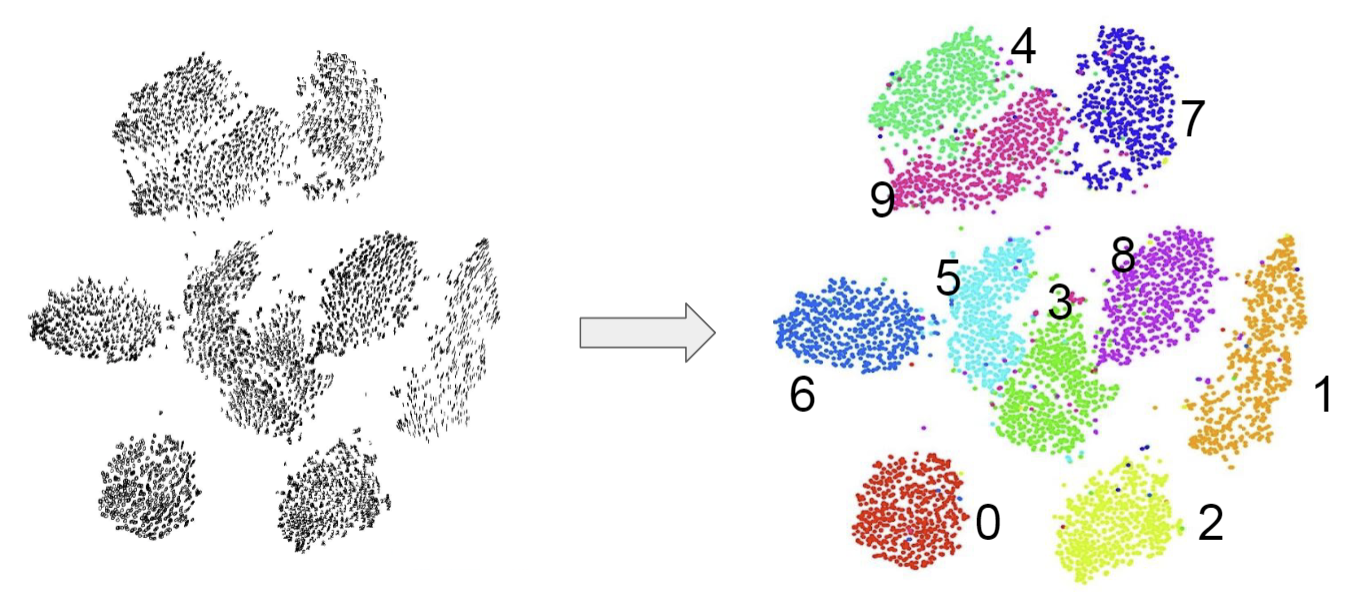
\includegraphics[width=0.5\linewidth]{featureclustering.png}
    \caption{Feature Clustering}
    \label{fig:enter-label}
\end{figure}

\begin{definition}
    \textbf{Unsupervised Learning:} learning patterns from data without human annotations (e.g., clustering, density estimation, dimensionality reduction).
\end{definition}

\begin{definition}
    \textbf{Self-supervised Learning:} use the success of supervised learning without relying on human provided
supervision (automatic supervision) (e.g., mask part of the input and predict the masked information).
\end{definition}

\begin{definition}
    \textbf{Semi-supervised Learning:} learning from data that mostly consists of unlabeled samples. A small amount of human-labeled data is available as well.
\end{definition}

\section{Autoencoders}

\begin{definition}
    \textbf{Autoencoders:} neural network architectures designed for unsupervised learning. They consist of an encoder and a decoder network. The encoder compresses input data into a lower-dimensional representation (encoding), while the decoder reconstructs the original data from this encoding. The goal is to learn an efficient representation of the data, typically for tasks like data compression, denoising, or dimensionality reduction.
\end{definition}

Find efficient representations of input data that could be used to reconstruct the original input using two components:

\begin{itemize}
    \item \textbf{Encoder}
    \begin{itemize}
        \item Converts the inputs to an internal representation
    \end{itemize}
    \begin{itemize}
        \item Dimensionality reduction
    \end{itemize}
    \item \textbf{Decoder}
    \begin{itemize}
        \item Converts the internal representation to the outputs
    \end{itemize}
    \begin{itemize}
        \item Generative network
    \end{itemize}
\end{itemize}

The number of outputs is the same as the inputs.\textbf{ Hourglass shape creates a bottleneck layer}, lowering dimensional representation. Similar to ANNs and CNNs, we use a loss function to quantify reconstruction error.

\begin{figure}[h!t]
    \centering
    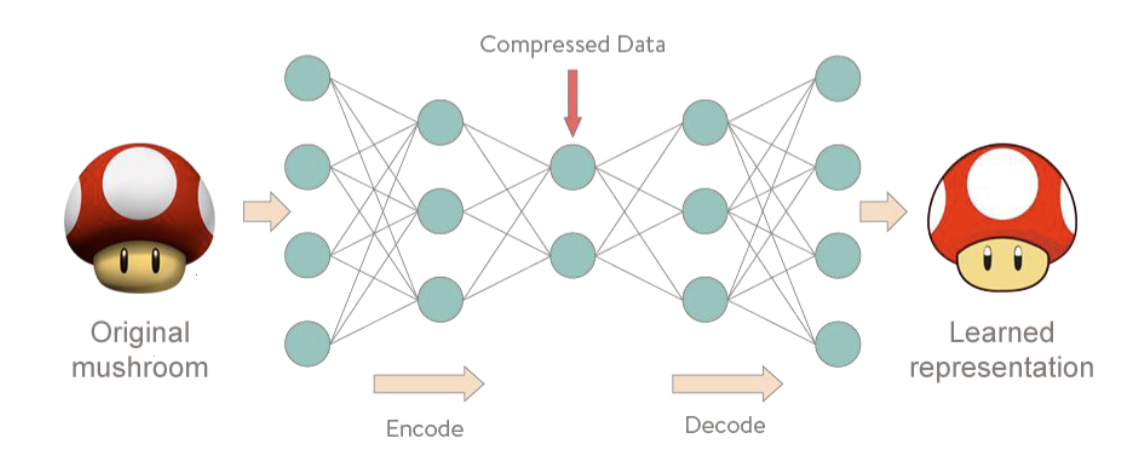
\includegraphics[width=0.6\linewidth]{hourglass.png}
    \caption{Hourglass shape of an Autoencoder}
    \label{fig:enter-label}
\end{figure}

The autoencoder is forced to learn the most important features in the input data and drop the unimportant ones.
\begin{figure}[h!t]
    \centering
    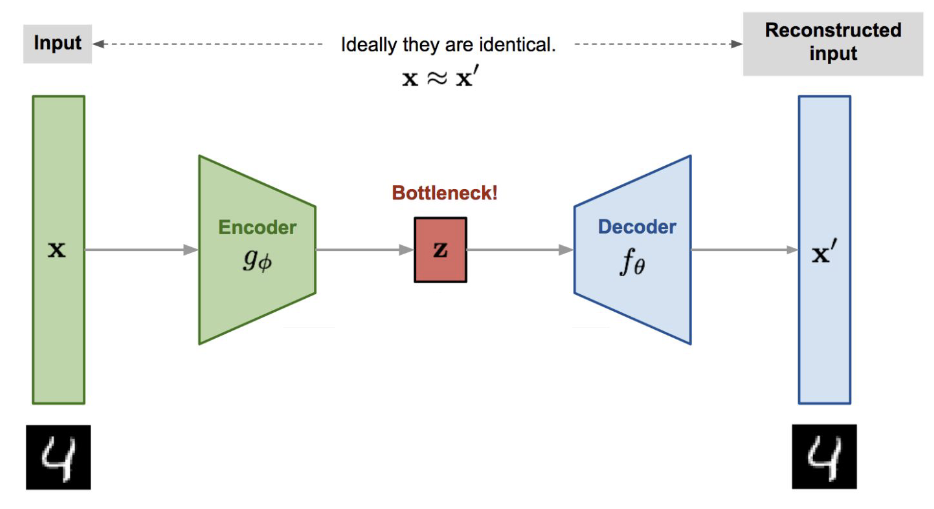
\includegraphics[width=0.65\linewidth]{Autoencoder.png}
    \caption{Autoencoder structure}
    \label{fig:enter-label}
\end{figure}


\newpage
\textbf{Applications}
\begin{itemize}
    \item Feature Extraction
    \item Unsupervised Pre-training
    \item Dimensionality Reduction
    \item Generate new data
    \item Anomaly detection → Autoencoders are bad at reconstructing outliers\\
\end{itemize}

\begin{figure}[h!t]
    \centering
    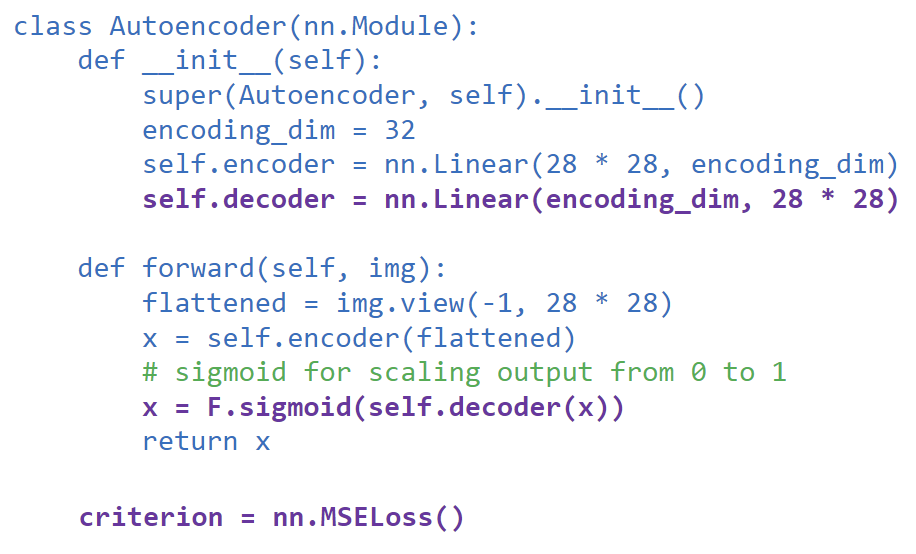
\includegraphics[width=0.5\linewidth]{autoencoderpy.png}
    \caption{Simple PyTorch Implementation of an Autoencoder}
    \label{fig:enter-label}
\end{figure}

\textbf{Stacked Autoencoders}
\begin{itemize}
    \item Autoencoders can have multiple hidden layers: stacked (deep) autoencoders
    \item Typically symmetrical with regards to the central coding layer.
\end{itemize}

\begin{figure}[h!t]
    \centering
    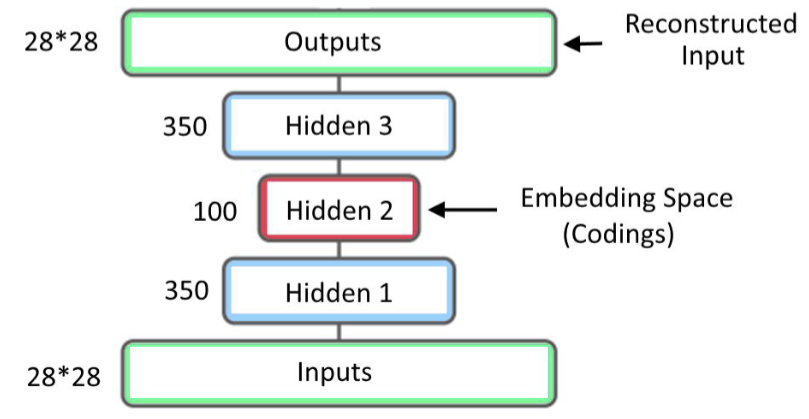
\includegraphics[width=0.55\linewidth]{stackedautoencoders.png}
    \caption{Stacked Autoencoders}
    \label{fig:enter-label}
\end{figure}

\textbf{Visualizing Reconstructions:} a way to ensure that an autoencoder is properly trained is to compare the inputs and the outputs.

\begin{figure}[h!t]
    \centering
    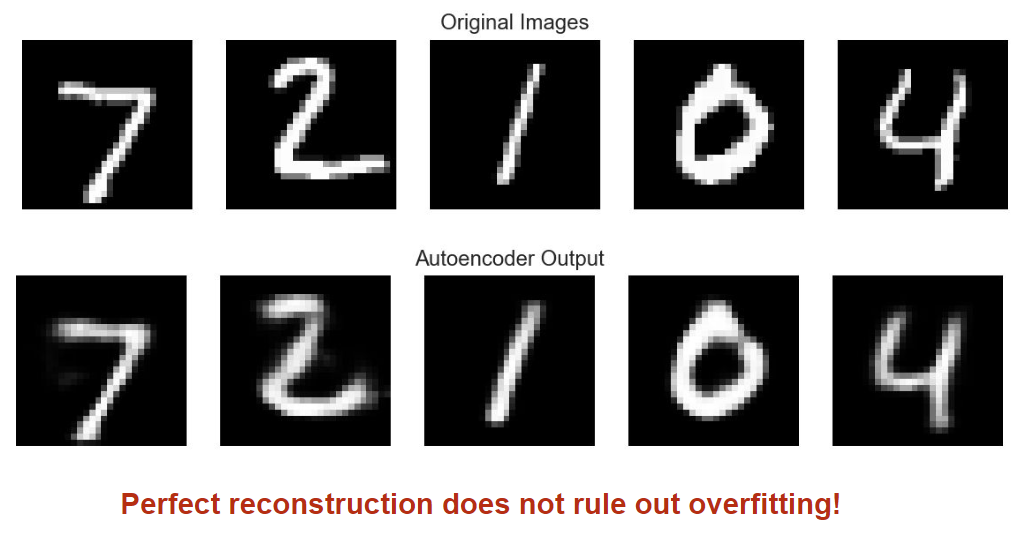
\includegraphics[width=0.45\linewidth]{visualizeautoencoder.png}
    \caption{Visualizing autoencoder reconstructions}
    \label{fig:enter-label}
\end{figure}
\newpage

\begin{idea}
    Autoencoders often have issues with overfitting. We can help mitigate this problem using denoising autoencoders.
\end{idea}

\textbf{Denoising Autoencoders}
\begin{itemize}
    \item Noise can be added to the input images of the autoencoder to force it to learn useful features (regularization)
\item Autoencoder is trained to recover the original, noise-free inputs.
\item Prevents it from trivially copying its inputs to its outputs, has to find patterns in the data.
\item Two common ways:
\begin{itemize}
    \item Adding gaussian noise (salt and pepper effect)
    \item Randomly masking inputs (dropout for pixels)
\end{itemize}
\end{itemize}

\begin{figure}[h!t]
    \centering
    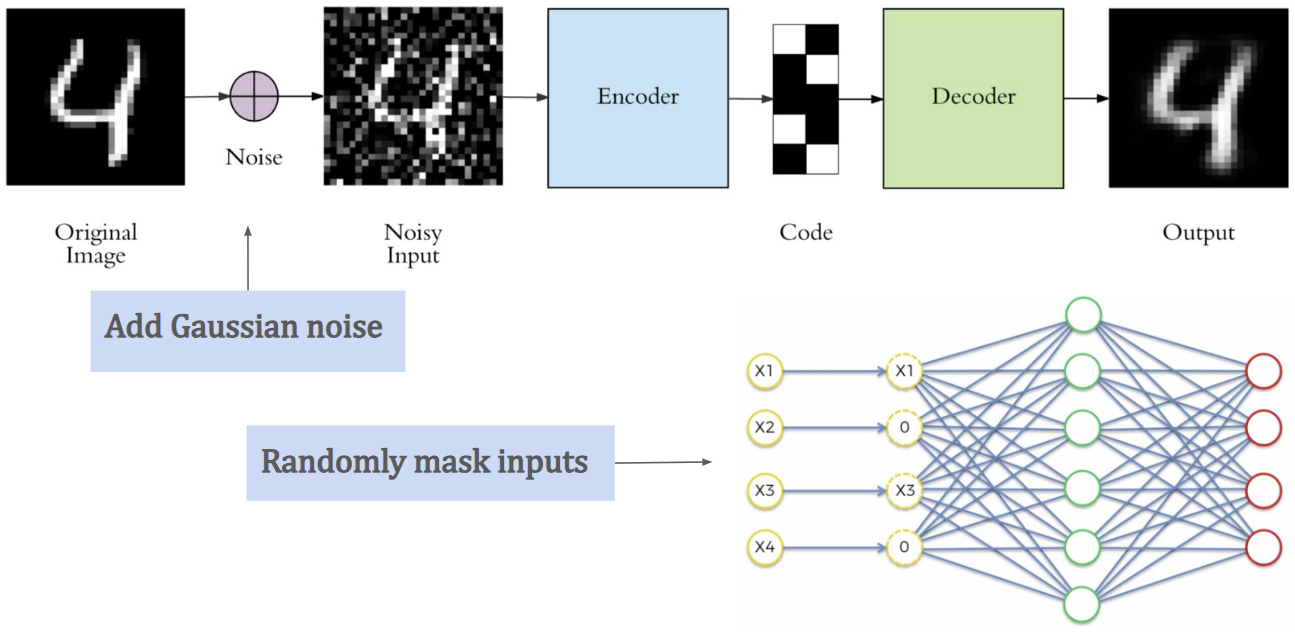
\includegraphics[width=0.5\linewidth]{denoiseautoencoders.png}
    \caption{Ways to denoise autoencoders}
    \label{fig:enter-label}
\end{figure}

\begin{figure}[h!t]
    \centering
    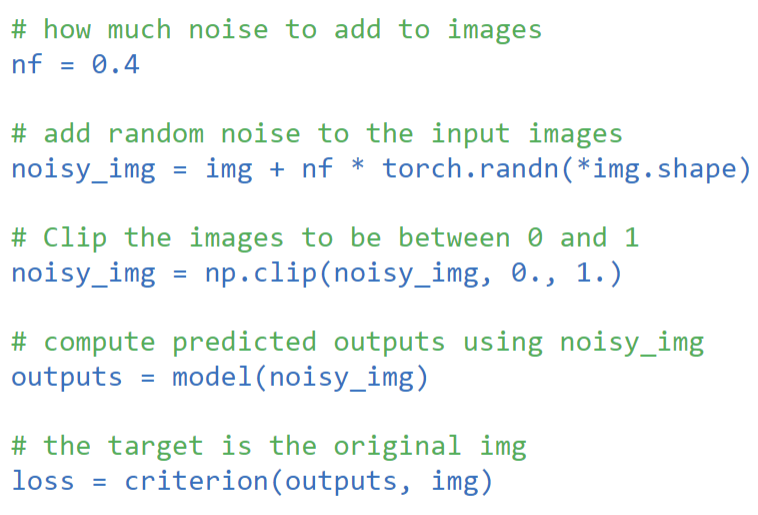
\includegraphics[width=0.4\linewidth]{gaussiannoisepy.png}
    \caption{PyTorch implementation of Gaussian noise}
    \label{fig:enter-label}
\end{figure}

\begin{figure}[h!t]
    \centering
    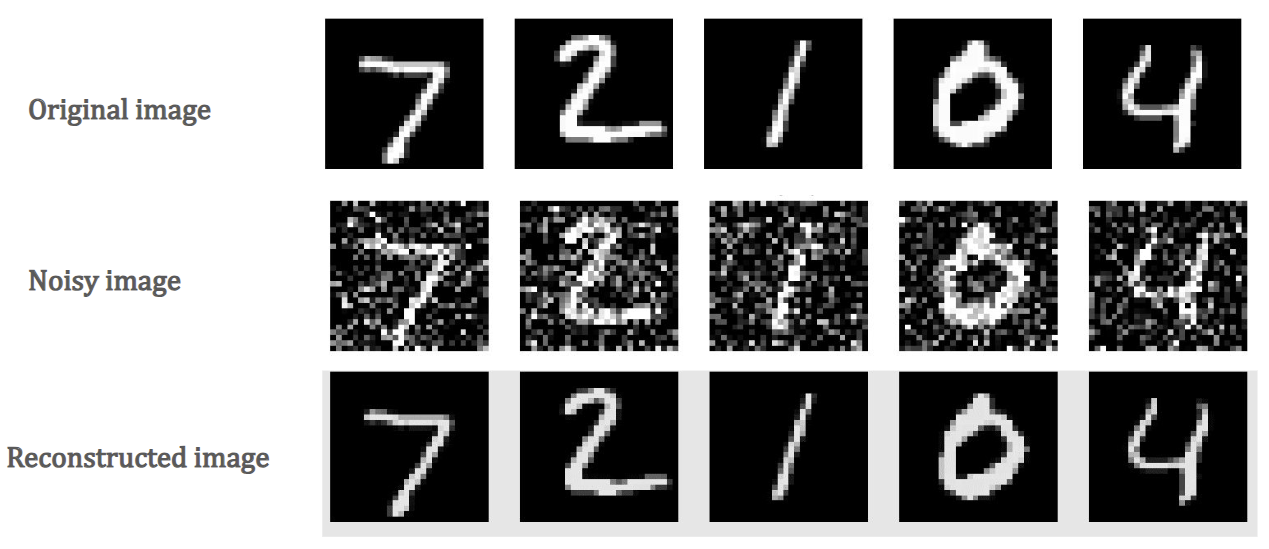
\includegraphics[width=0.4\linewidth]{effectofaddingnoise.png}
    \caption{Visualization of adding Gaussian noise to autoencoders}
    \label{fig:enter-label}
\end{figure}

\textbf{Generating New Images}

\begin{itemize}
    \item Since we are drastically reducing the dimensionality of the image, there has to be
some kind of structure in the codings (i.e. embedding space)
\item That is, the network should be able to save space by mapping similar images to
similar embeddings
\item Let’s see how we can exploit this to allow us to generate new types of images which can be used to create a more robust and vast dataset
\end{itemize}

\textbf{New Images with Interpolation}
\begin{enumerate}
    \item First compute low-dimensional embeddings of two images.
    \item Then interpolate between the two embeddings and decode those as well!
    \item Interpolated codings result in new images that are somewhere in between the two starting images.
\end{enumerate}

\begin{figure}[h!t]
    \centering
    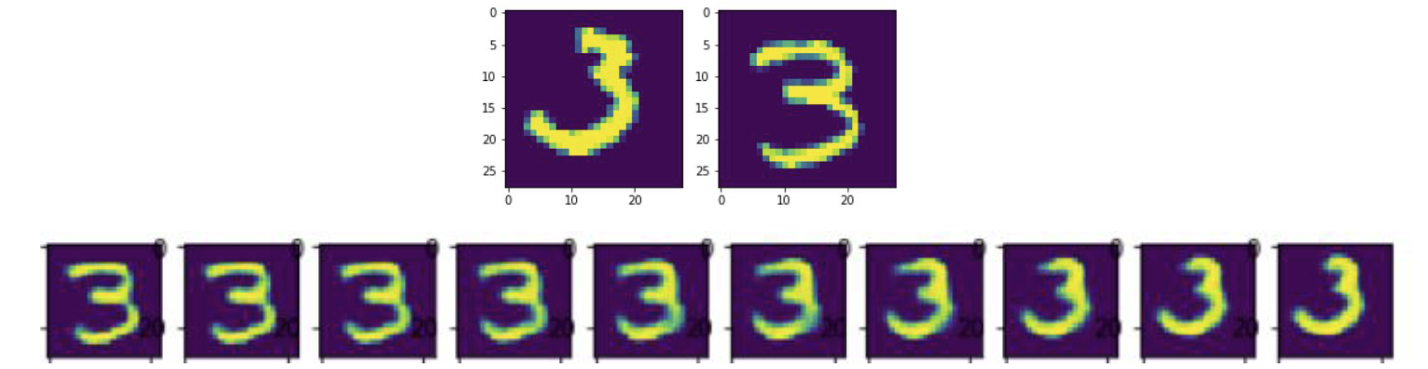
\includegraphics[width=0.75\linewidth]{interpolationex.png}
    \caption{Combining embeddings using Interpolation}
    \label{fig:enter-label}
\end{figure}

\textbf{What if we randomly select a coding?}: The latent space in autoencoders can become disjoint and non-continues (looks like the input but is actually nonsense). Very rarely, the random number might acrually generate a meaningul (actual) digit, but this is unlikely due to the high number of dimensions.

\begin{figure}[h!t]
    \centering
    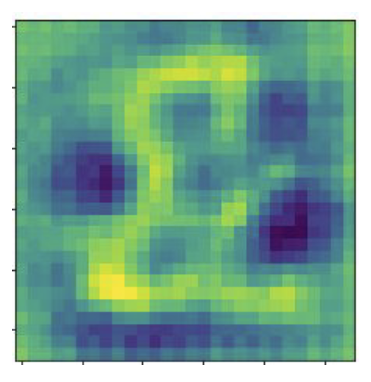
\includegraphics[width=0.15\linewidth]{randomcoding.png}
    \caption{Randomly selecting a coding}
    \label{fig:enter-label}
\end{figure}

\begin{idea}
   Denoising autoencoders often have issues with the smoothness of the embedding space. We can help mitigate this problem using variational autoencoders.
\end{idea}

\section{Variational Autoencoders}

\begin{definition}
    \textbf{Variational Autoencoders:} probabilistic generative models that consist of an encoder and a decoder neural network. VAEs aim to learn a probabilistic mapping between the input data and a latent space, where data points are represented as probability distributions. Unlike traditional autoencoders, VAEs generate data points by sampling from these distributions, making them useful for generating new data samples and data generation tasks. VAEs are often used in tasks such as image generation, data synthesis, and data denoising.
\end{definition}

\begin{figure}[h!t]
    \centering
    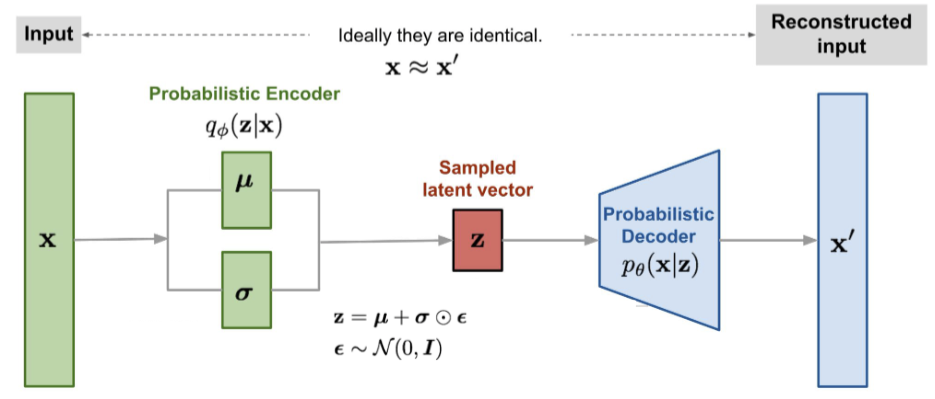
\includegraphics[width=0.5\linewidth]{vae.png}
    \caption{Variational autoencoder structure}
    \label{fig:enter-label}
\end{figure}

They are quite different from the autoencoders we have discussed so far:
\begin{itemize}
    \item \textbf{Probabilistic} → their outputs are partly determined by chance even after training (the same input will not always yield the same results every time)
    \item \textbf{Generative }→ they can generate (an infinite number of) new instances that look like they were sampled from the training set, but are not the same as the training set.
\end{itemize}
They impose a distribution constraint on the latent space to have a smooth space.\\

\begin{figure}[h!t]
    \centering
    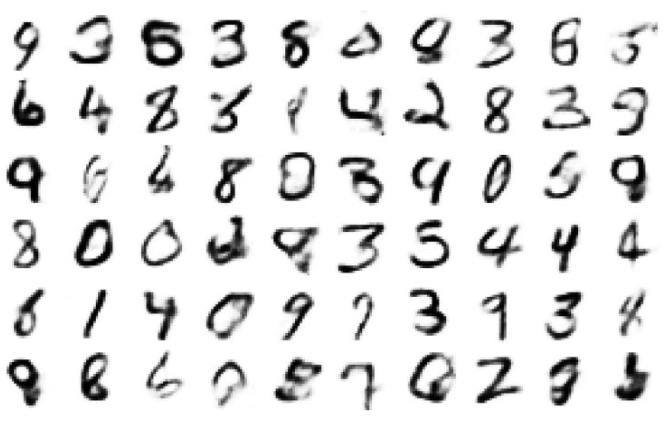
\includegraphics[width=0.35\linewidth]{generativeVae.png}
    \caption{Generated images that look like handwritten digits by training a variational autoencoder}
    \label{fig:enter-label}
\end{figure}

\begin{definition}
    \textbf{Gaussian Distribution:} also known as a normal distribution, is a probability distribution that is characterized by its bell-shaped curve. It is defined by two parameters: the mean (\(\mu\)), which represents the center of the distribution, and the standard deviation (\(\sigma\)), which measures the spread or dispersion of the data. In a Gaussian distribution, data tends to cluster around the mean, with the majority of values close to the mean, and it follows a symmetrical pattern.
\end{definition}

\textbf{Encoder generates a normal distribution with mean \(\mu\) and a standard deviation \(\sigma\) instead of a fixed embedding.} An embedding is sampled from the distribution and decoder decodes the sample to
reconstruct the input.

We want the encoder distribution \( q_\phi (z|x) = N(\mu, \sigma)\) to be close prior \( p(z) = N(0, I)\). We can use Kullback-Leibler (KL) divergence to measure the difference between two distributions P(X) and and Q(X):
\[ D_{KL}(P||Q) = \sum_{x \in X}p(x)log(\frac{p(x)}{q(x)})\]

If we plug in the encoder distrubution and the prior KL-divergence of two multivariate Gaussians, we get: 

\[ D_{KL}(p|q) = \frac{1}{2} \sum_{i = 1}^{N}[\mu^2_i + \sigma^2_i - (1 + log(\sigma^2_i))] \]

\begin{figure}[h!t]
    \centering
    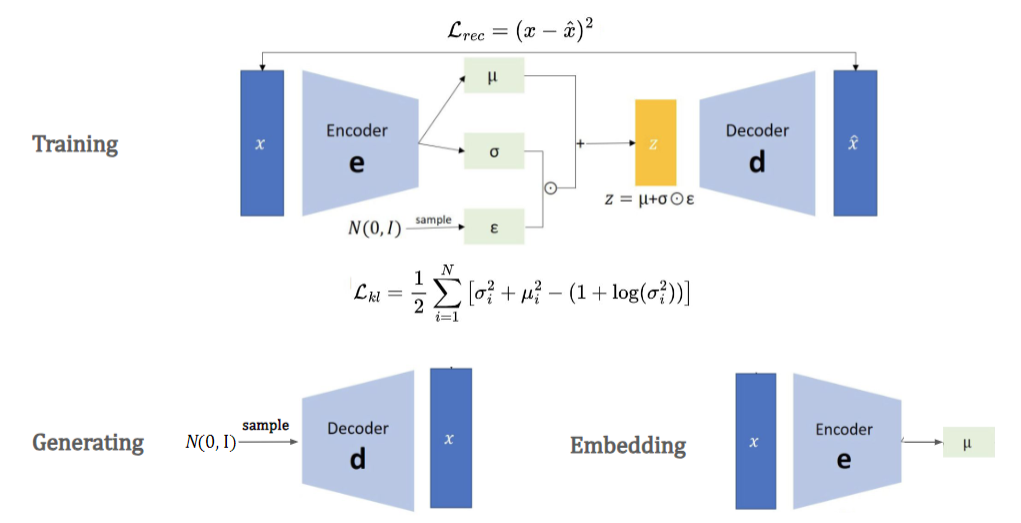
\includegraphics[width=0.55\linewidth]{vae2.png}
    \caption{Variational autoencoders: training, generating, and embedding}
    \label{fig:enter-label}
\end{figure}

\begin{idea}
    Generating new images requires that we sample a latent vector from the unit Gaussian and pass it into the decoder. Variational autoencoders use probability distribution for embeddings such that the entirety of the embeddings subspace is valid input to the decoder. Basically, to ensure that the output from an encoder is not nonsense.
\end{idea}

\section{Convolutional Autoencoders}

\begin{idea}
    When it comes to dealing with images, convolution is much better than fully connected networks.
\end{idea}

\begin{definition}
   \textbf{Convolutional Autoencoders:} a type of artificial neural network designed for unsupervised learning that uses convolutional layers to encode and decode input data efficiently. It is primarily used for feature extraction and dimensionality reduction in tasks such as image reconstruction and denoising.
\end{definition}

\begin{figure}[h!t]
    \centering
    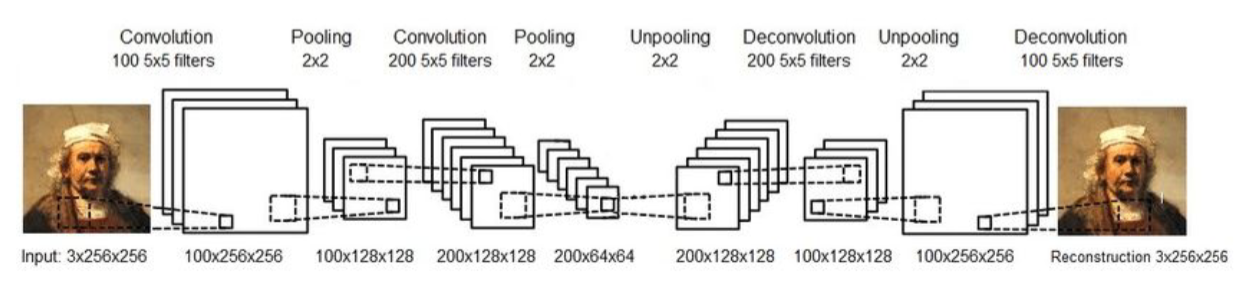
\includegraphics[width=0.75\linewidth]{convautoencoder.png}
    \caption{Convolutional autoencoder}
    \label{fig:enter-label}
\end{figure}

\textbf{Convolutional autoencoders take advantage of spatial information.}
\begin{itemize}
    \item \textbf{Encoder} → Learns visual embedding using convolutional layers
    \item \textbf{Decoder} → Up-samples the learned visual embedding to match the original size of the image.
\end{itemize}

\begin{definition}
    \textbf{Transposed Convolution:} also known as "deconvolutions" or "up-sampling," are operations in deep learning that expand the spatial dimensions of data, typically in convolutional neural networks, by using learnable filters to perform upsampling or interpolation, allowing the network to generate higher-resolution feature maps from lower-resolution input.
\end{definition}

The opposite of the convolution is the\textbf{ transposed convolution} (different from an
inverse convolution). They work with filters, kernels, padding, strides just as the convolution layers. Instead of mapping KxK pixels to 1, they can map from 1 pixel to KxK pixels. The kernels are learned just like normal convolutional kernels.


\begin{theorem}
    \textbf{Computing the output size of the feature map (from transpose convolving an image with a kernel)}\\

For each dimension of an input image with:
\begin{itemize}
    \item Image dimension of size \textbf{i}
    \item Kernel of size \textbf{k}
    \item Padding of size \textbf{p}
    \item Output padding of size \textbf{op}
    \item Stride of size \textbf{s}
\end{itemize}
The size of output dimension is computed by:


\[o = (i - 1) \cdot s + (k - 1) - 2p + op + 1 \]

\end{theorem}

\textbf{To perform transposed convolution:}
\begin{enumerate}
    \item Take each pixel of your input image
    \item Multiply each value of your kernel with the input pixel to get a weighted kernel
    \item Insert it in the output to create an image
\begin{figure}[h!t]
    \centering
    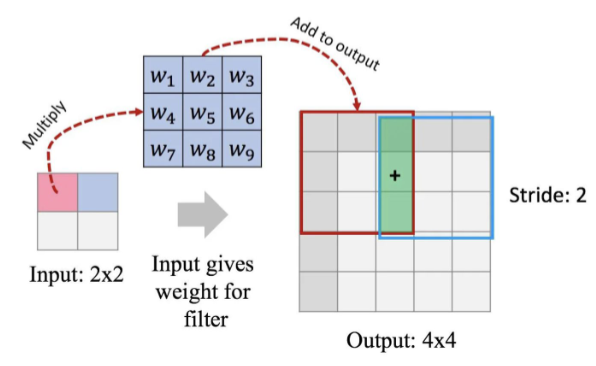
\includegraphics[width=0.45\linewidth]{tconv1.png}
    \caption{Transposed Convolution}
    \label{fig:enter-label}
\end{figure}
    \item Where the outputs overlap, sum them
\end{enumerate}
\begin{figure}[h!t]
    \centering
    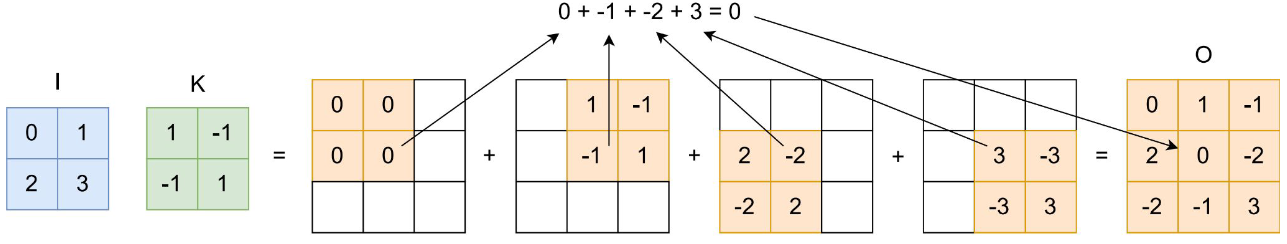
\includegraphics[width=0.75\linewidth]{tconv2.png}
    \caption{Transposed Convolution}
    \label{fig:enter-label}
\end{figure}

\newpage

\textbf{Padding} \\
\indent The effect is the opposite of what happens with the convolution layers:
\begin{itemize}
    \item Compute the output as normal
    \item Remove rows and columns around the perimeter
\end{itemize}

\begin{figure}[h!t]
    \centering
    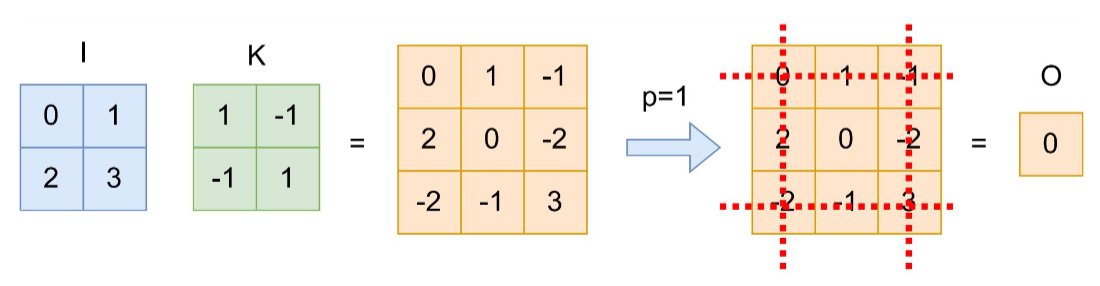
\includegraphics[width=0.75\linewidth]{paddingtconv.png}
    \caption{Padding in transposed convolution}
    \label{fig:enter-label}
\end{figure}

\textbf{Output Padding}

\begin{itemize}
    \item When stride $> 1$, \texttt{Conv2d} maps multiple input shapes to the same output shape.
    \item E.g. Inputs of size $7 \times 7$ and $8 \times 8$ both return an output of $3 \times 3$ for a kernel of size $3 \times 3$ with \texttt{stride}$=2$.
    \item When applying the transpose convolution, it is ambiguous which output shape to return, $7 \times 7$ or $8 \times 8$ for \texttt{stride}$=2$ transpose convolution.
    \item Output padding is provided to resolve this ambiguity by effectively increasing the calculated output shape on one side.
    \item It is only used to find the output shape but does not actually add zero-padding to the output.
\end{itemize}

\textbf{Strides}
\begin{itemize}
    \item The effect is also the opposite from what happens with the convolution layers
    \item Increasing the stride results in an increase in the upsampling effect.
\end{itemize}

\begin{figure}[h!t]
    \centering
    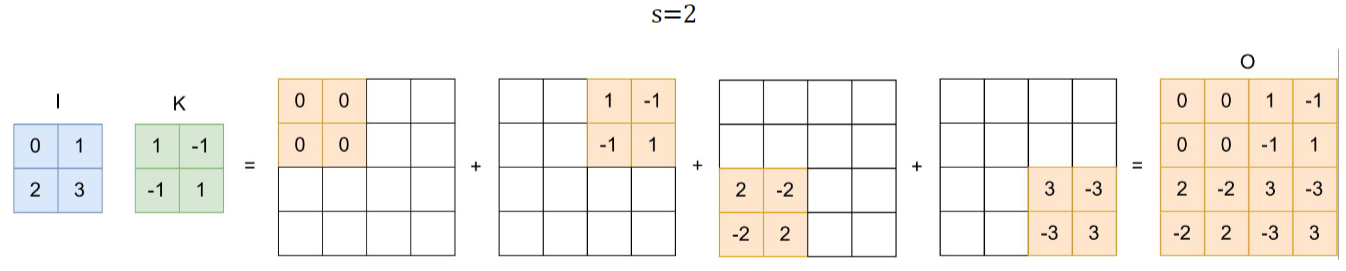
\includegraphics[width=0.75\linewidth]{stridesconvae.png}
     \caption{Strides in transposed convolution}
    \label{fig:enter-label}
\end{figure}

A convolution transpose layer with the exact same specifications as the convolution
layer would have the reverse effect on the shape.

\begin{figure}[h!t]
    \centering
    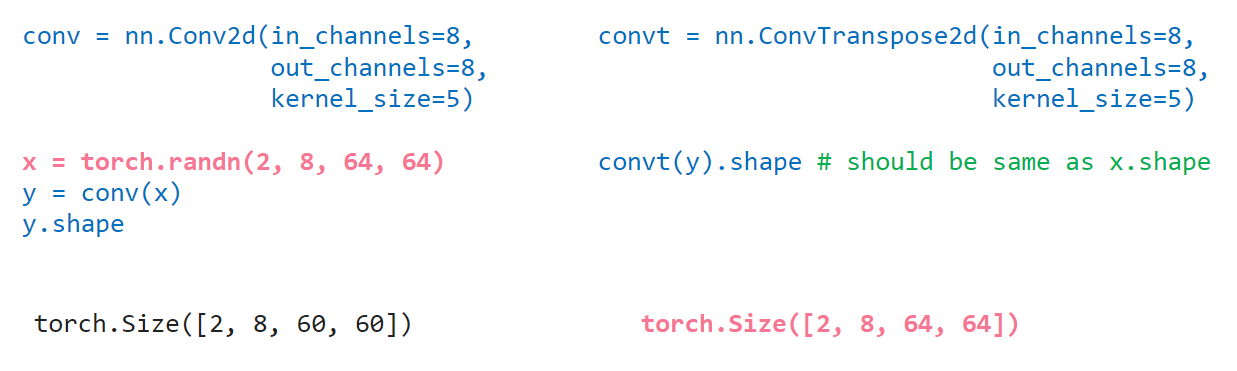
\includegraphics[width=0.5\linewidth]{convandtconv.png}
    \caption{PyTorch implementation of convolution and transposed convolution}
    \label{fig:enter-label}
\end{figure}

\newpage

We also have the option of including convolution transpose padding:

\begin{figure}[h!t]
    \centering
    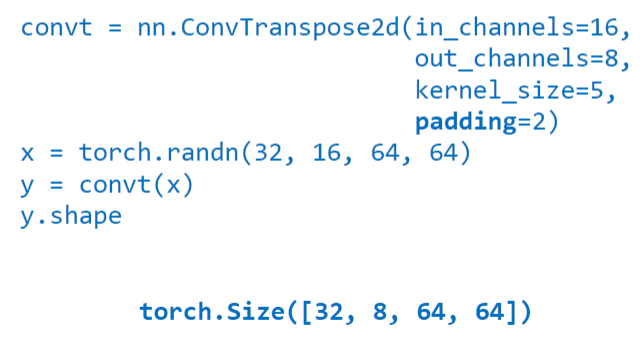
\includegraphics[width=0.35\linewidth]{tpadding.png}
    \caption{Transpose padding in PyTorch}
    \label{fig:enter-label}
\end{figure}

We can add a stride to the convolution to increase our resolution!

\begin{figure}[h!t]
    \centering
    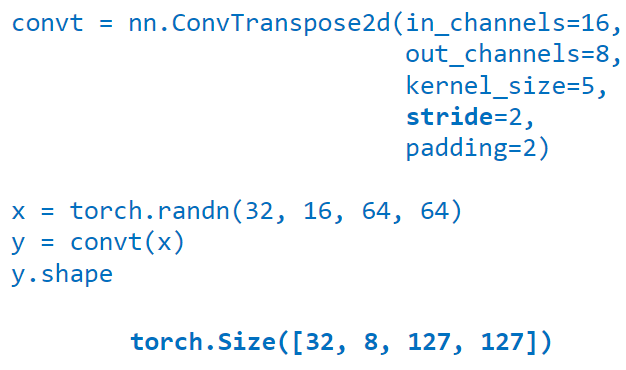
\includegraphics[width=0.35\linewidth]{stridetconv.png}
    \caption{Transpose stride in PyTorch}
    \label{fig:enter-label}
\end{figure}

Output padding is another type of padding that adds an additional row and column to the output. It's easy to mix it up with padding.

\begin{figure}[h!t]
    \centering
    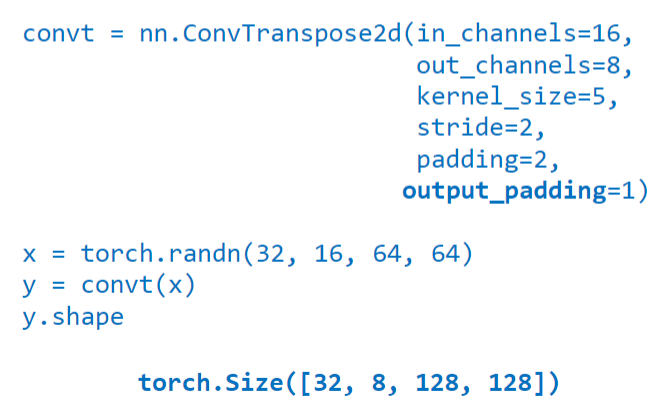
\includegraphics[width=0.35\linewidth]{outputpaddingtconv.png}
    \caption{Output padding in PyTorch}
    \label{fig:enter-label}
\end{figure}


\begin{idea}
    \textbf{PyTorch Implementation of convolutional autoencoder:}

\begin{verbatim}
class Autoencoder(nn.Module):
    def __init__(self):
        super(Autoencoder, self).__init__()
        self.encoder = nn.Sequential(
            nn.Conv2d(1, 16, 3, stride=2, padding=1),
            nn.ReLU(),
            nn.Conv2d(16, 32, 3, stride=2, padding=1),
            nn.ReLU(),
            nn.Conv2d(32, 64, 7)
        )
        self.decoder = nn.Sequential(
            nn.ConvTranspose2d(64, 32, 7),
            nn.ReLU(),
            nn.ConvTranspose2d(32, 16, 3, stride=2, padding=1, output_padding=1),
            nn.ReLU(),
            nn.ConvTranspose2d(16, 1, 3, stride=2, padding=1, output_padding=1),
            nn.Sigmoid()
        )

        def forward(self, x):
            x = self.encoder(x)
            x = self.decoder(x)
            return x

        def embed(self, x):
            return self.encoder(x)

        def decode(self, e):
        return self.decoder(e)
\end{verbatim}
\end{idea}

\section{Pre-training with Autoencoders}

Previously we discussed how transfer learning could use features obtained from ImageNet data to improve classification on other image tasks.
\begin{itemize}
    \item Assumption that the ImageNet data is similar in the new task.
    \item If the new task is to detect new objects from similar images, then transfer learning makes sense.
\end{itemize}
Autoencoders can achieve similar results by pretraining on large set of unlabeled data, same type of data, just missing labels.

\begin{figure}[h!t]
    \centering
    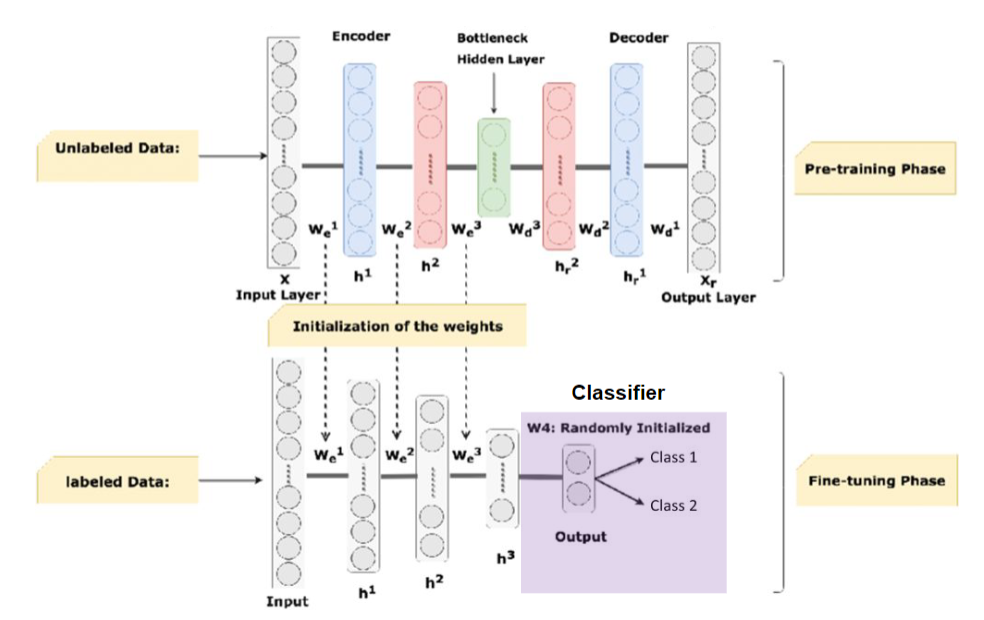
\includegraphics[width=0.6\linewidth]{pretrainae.png}
    \caption{Pre-training Autoencoders}
    \label{fig:enter-label}
\end{figure}

\section{Self-Supervised Learning}

What if we can cast unsupervised learning into supervised setting? \textbf{Define proxy supervised tasks such that:}
\begin{itemize}
    \item The labels are generated automatically for free (utilizing advantage of no human input here)
    \item Solving the task, requires the model to “understand” the content
\end{itemize}
The challenge is devising the tasks such that they enforce the model to learn robust
representations.\\

\newpage

\noindent\textbf{RotNet}

\begin{definition}
     \textbf{RotNet:} architecture designed for the task of image rotation recognition. It is trained to predict the rotation angle of an input image, typically in 90-degree increments (0°, 90°, 180°, or 270°). RotNet helps improve the robustness of machine learning models by enabling them to recognize objects in images regardless of their orientation, which can be useful in various computer vision applications.
\end{definition}

\begin{idea}
    Rotate images randomly by 0, 90, 180, or 270 degrees and make the model to
predict the rotation angle.
\end{idea}

\begin{figure}[h!t]
    \centering
    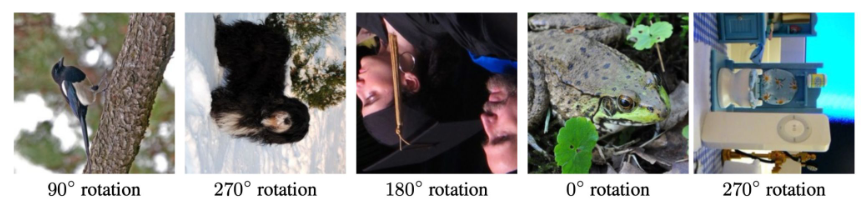
\includegraphics[width=0.75\linewidth]{rotnet.png}
    \caption{Rotating images and keeping rotations as ground truth labels assigned by program}
    \label{fig:enter-label}
\end{figure}

If someone is not aware of the concepts of the objects depicted in the images, they
cannot recognize the rotation that was applied to them.

\begin{figure}[h!t]
    \centering
    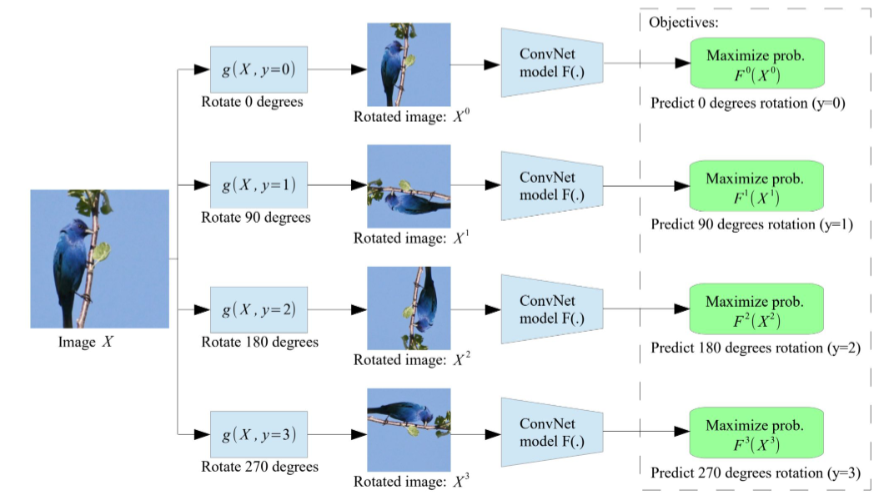
\includegraphics[width=0.6\linewidth]{rotnetclassification.png}
    \caption{RotNet Multiclass Classification}
    \label{fig:enter-label}
\end{figure}

\newpage

The task is multi-class classification with 4 classes (therefore cross-entropy loss) with free labels being generated automatically. \textbf{The disadvantage is that the task is still human-generated and needs to be "interesting" enough.} Otherwise, the network is going to cheat. Because of this, people moved to contrastive learning.\\

\noindent\textbf{Contrastive Learning}

\begin{definition}
    \textbf{Contrastive Learning:} a self-supervised learning technique in machine learning and deep learning, where a neural network is trained to differentiate between pairs of data points, typically by maximizing the similarity (or minimizing the distance) between positive pairs (similar data points) and minimizing the similarity (or maximizing the distance) between negative pairs (dissimilar data points). This approach is often used for feature learning and representation learning, where it helps the network learn meaningful and discriminative representations of data without the need for labeled data.

\end{definition}


\begin{table}[h!t]
\centering

\begin{tabular}{|p{8cm}|p{8cm}|}
\hline
\textbf{Autoencoding Methods} & \textbf{Contrastive Learning} \\
\hline
\begin{itemize}
  \item Reconstruct input
  \item Compute the loss in output space
  \item Compress all the details
\end{itemize}
&
\begin{itemize}
  \item Contrast pair of positive/negative samples
  \item Compute the loss in embedding space
  \item Compress relevant information
  \item Requires lots of negative examples
\end{itemize}
\\
\hline
\end{tabular}
\caption{Comparison: Autoencoding vs. Contrastive Learning}
\end{table}

\begin{figure}[h!t]
    \centering
    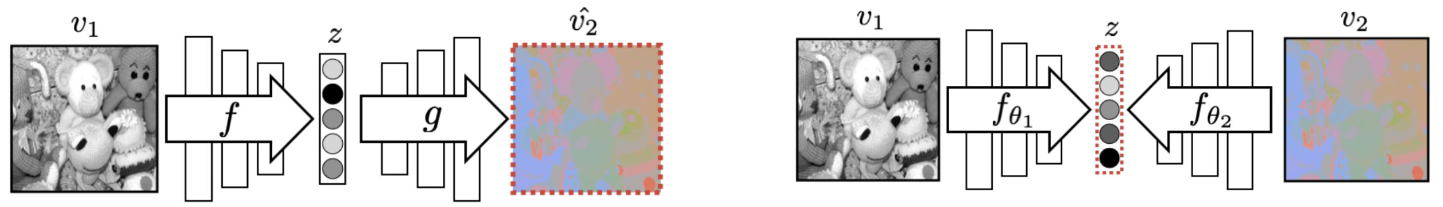
\includegraphics[width=1\linewidth]{autovscon.png}
    \caption{Autoencoding vs. Contrastive Learning}
    \label{fig:enter-label}
\end{figure}

\newpage

\textbf{SimCLR}

\begin{definition}
    \textbf{SimCLR:} short for "Simultaneous Contrastive Learning," is a self-supervised deep learning framework for learning powerful representations from unlabeled data. It is designed to encourage the model to pull together similar data points (positive pairs) while pushing apart dissimilar ones (negative pairs) in a high-dimensional feature space. SimCLR has been influential in achieving state-of-the-art results in various computer vision tasks by training on large datasets without the need for manual labeling.
\end{definition}

\begin{itemize}
    \item Augmentations of the same image are positive examples
    \item Augmentations of different images are negative examples
    \item \textbf{Same images are pushed together, different images are pushed away}
\end{itemize}

\begin{figure}[h!t]
    \centering
    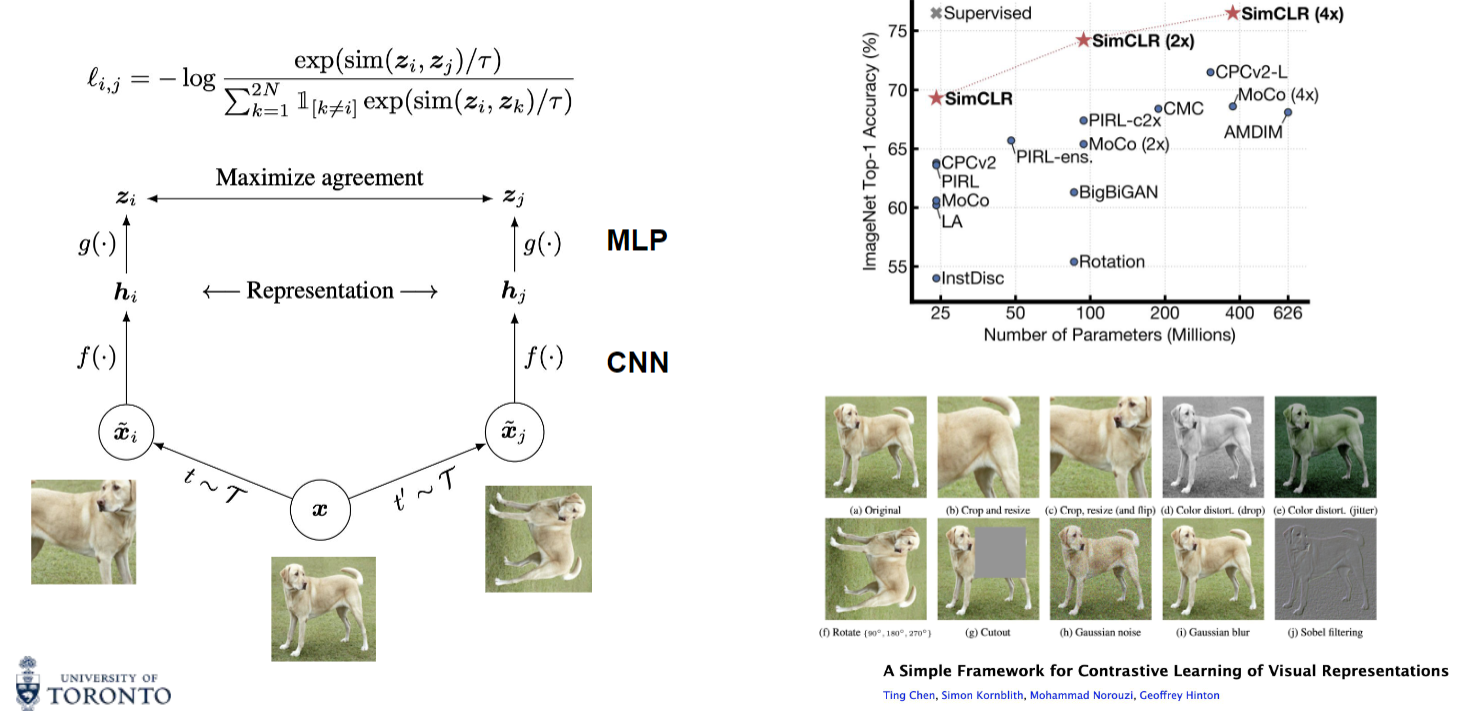
\includegraphics[width=0.9\linewidth]{simclr.png}
    \caption{SimCLR}
    \label{fig:enter-label}
\end{figure}
